\chapter{Conclusions}
\label{ch:conclusions}

The project aimed to:
\begin{itemize}
    \item Classify social media posts
    \item Quantify and compare a users social media feed to the rest of the social media site to identify interests
    \item Build a user interface that allows users to discover what their social media feed says about their interests and how they compare to the rest of the social media site
    \item Build a user interface to allow users to find posts that are dissimilar to the posts they are shown
\end{itemize}

It is clear that all of these aims were met. RoBERTa was fine-tuned for the topic classification task. The fine-tuning was done
using labelled data from Reddit and Wikipedia. Quantification of a set of tweets was done using the mean of the probabilistic outputs
from our model. A user interface was built that is able to show a comparison of topics between a users social media feed and the rest
of the social media site. The user interface also allows users to discover posts that are dissimilar to the posts they are shown.\\
From this, we can conclude that the project was a success.
\section{Future work}
\subsection{Advanced Context Input}
During this project the use of context was limited to media that was text based and comments/threads. However, there is a lot more information that can
be used to improve accuracy of topic classification.\\
Key information such as author, location, and date can be used to add context to a post. For example, if a post is made by a politician, then the topic is
likely to be about politics whereas if the post is made by a sports star, then the topic is likely to be about sports. This information in itself will not
be $100\%$ accurate, as politicians and sport stars can post about other topics as well. However, this information still serves as extra context to the post.
Including this context, in a similar manner to how we included media and comments/threads, could improve the accuracy of the model.\\\\
Another method of improving the context aware part of the model is to create a more sophisticated method of incorporating the context data. Currently, the
media text and comments/threads text is concatenated with the post text. This is a very naive method for adding context. For the media, a possible improvement
could be to use transfer learning. This would allow us to extract more meaningful data from media and not just the text that is present in it. Transformers
have been used for image/video classification. It could be possible to train a transformer model on a dataset of images/videos
and then use the output (or possibly a feature vector) of this model as the context for the post. Transfer learning and 
concatenation of this model output with the RoBERTa model output could be used to create a new `context aware' model.
\begin{figure}
    \centering
    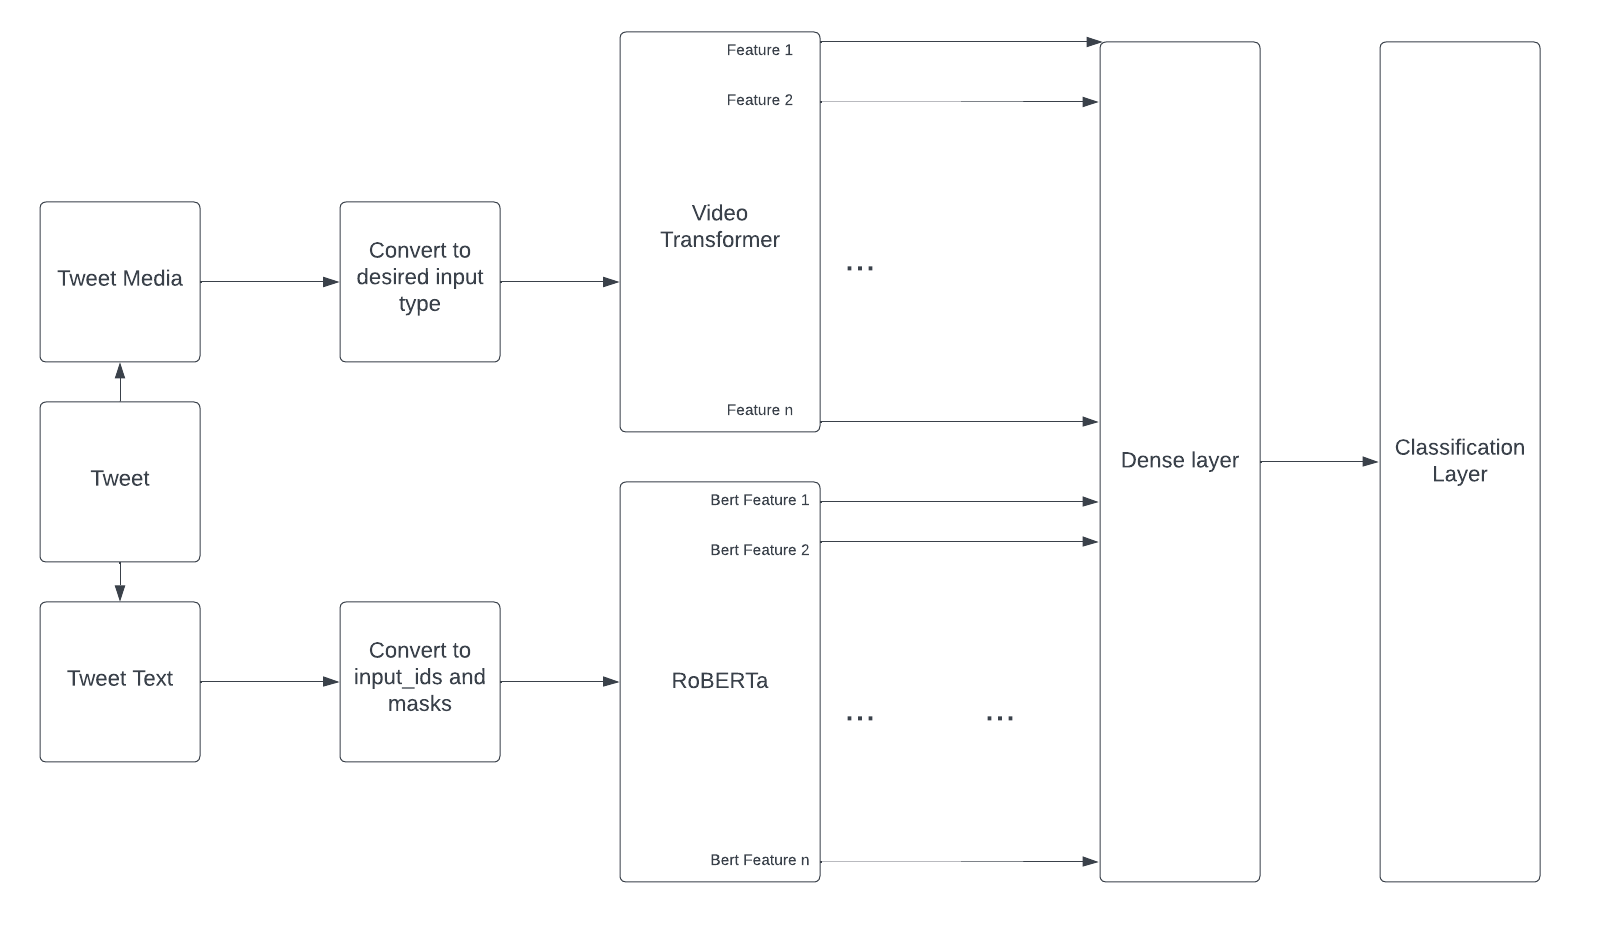
\includegraphics[width=0.5\textwidth]{images/transfer-learning.png}
    \caption{Transfer Learning with RoBERTa and Video Transformers}
    \label{fig:transfer-learning}
\end{figure}
As seen in Figure \ref{fig:transfer-learning}, The post text is fed through RoBERTa and the media is fed through Video Transformers. The outputs of both models
are fed through a linear layer seperately, and then concatenated together. This is then fed through a linear layer and a softmax layer to get the final output.
\subsection{Chrome Extension}
Originally, the project was going to create a chrome extension. However, due to the time constraints of the project and the fact that I have never worked
with JavaScript or Chrome extensions before, this was not possible. An extension to this project would be to learn these frameworks and transfer the
user interface to a chrome extension. This would give the application a better platform to be used on - chrome extension store.
\subsection{Bias Analysis}
When first developing the idea for this project the main aim was to be able to find bias in someones social media feed. The idea came from some reading
on echo chambers: ``an epistemic environment in which participants encounter beliefs and opinions that coincide with their own'' \cite{echo-chambers}.
An Echo chamber can cause individuals to be subject to posts that agree with their ideologies, whether or not they are `true' or `representative' of all viewpoints.
The notion of `bias' comes from the fact the posts that are shown are not truly representative of all viewpoints; the user is only shown posts that agree with their own.\\
This project is a good baseline for analysis on bias in a users social media feed. This project allows us to identfiy what topics a user is interested in. However, this
in itself does not gauge whether the feed is bias or not. A user may be interested in a topic and see posts that show all viewpoints on that topic. This is not bias.
However, if a user is only shown posts about one side/part of the given topic, then this can be construed as bias. For example, take a user who is interested in sports.
For this user to be non-bias they would need to see posts on a range of sports: Football, Rugby, Cricket, Ahthletics, and so on. However, if they only see posts on Football
this can be seen as bias towards football.\\
This project can be extended to find the differences within topics to identify bias that is present in a users social media feed. Some early ideas for this include:
\begin{itemize}
    \item Keyword analysis to find subtopics within a Topic.
    \item Building new models that given an overarching topic can identify subtopics.
\end{itemize}